\section{Interfejs użytkownika (Zofia Sosińska)}\label{chap:ui}
Interfejs użytkownika (ang. user interface, UI) jest to zbiór najważniejszych informacji przedstawiony graczowi w sposób czytelny. Może się to odbywać za pomocą na przykład obrazków, tekstów, czy wskaźników. Dzięki UI możliwy jest wgląd w aktualny stan wiedzy grywalnej postaci. 

Projekt interfejsu użytkownika przewiduje trzy tryby: zwykły, budowania oraz walki. Zadaniem każdego z nich będzie odzwierciedlenie aktualnej wiedzy granej postaci z naciskiem na najpotrzebniejsze w danej chwili informacje.
	
\subsection{Interfejs podstawowy}
Interfejs podstawowy przewiduje funkcje, takie jak pokazanie:
\begin{itemize}
    \item surowców i funduszy,
    \item aktualnego czasu w grze, 
    \item kompasu,
    \item informacji o możliwym  rozpoczęciu konwersacji z inną postacią;
\end{itemize}
Inspiracją dla górnego paska z informacjami jest ten użyty w grze Warcraft 3. Prostota i surowość stylu będą współgrać z klimatem gry.

W naszej grze skupimy się jednak na tym, aby interfejs użytkownika zabierał jak najmniej miejsca. Dlatego też projekt zakłada, że poszczególne obiekty nie będą ze sobą połączone, a jedynie “dryfować” w przestrzeni.
Jako ważny element tej części UI zawarty zostanie kompas, wzorowany na tym z gry The Elder Scrolls V: Skyrim.


Szacowany projekt interfejsu podstawowego UI wyświetlono na rysunku \ref{fig:ui_main} .
\begin{figure}[htbp]
    \centering
    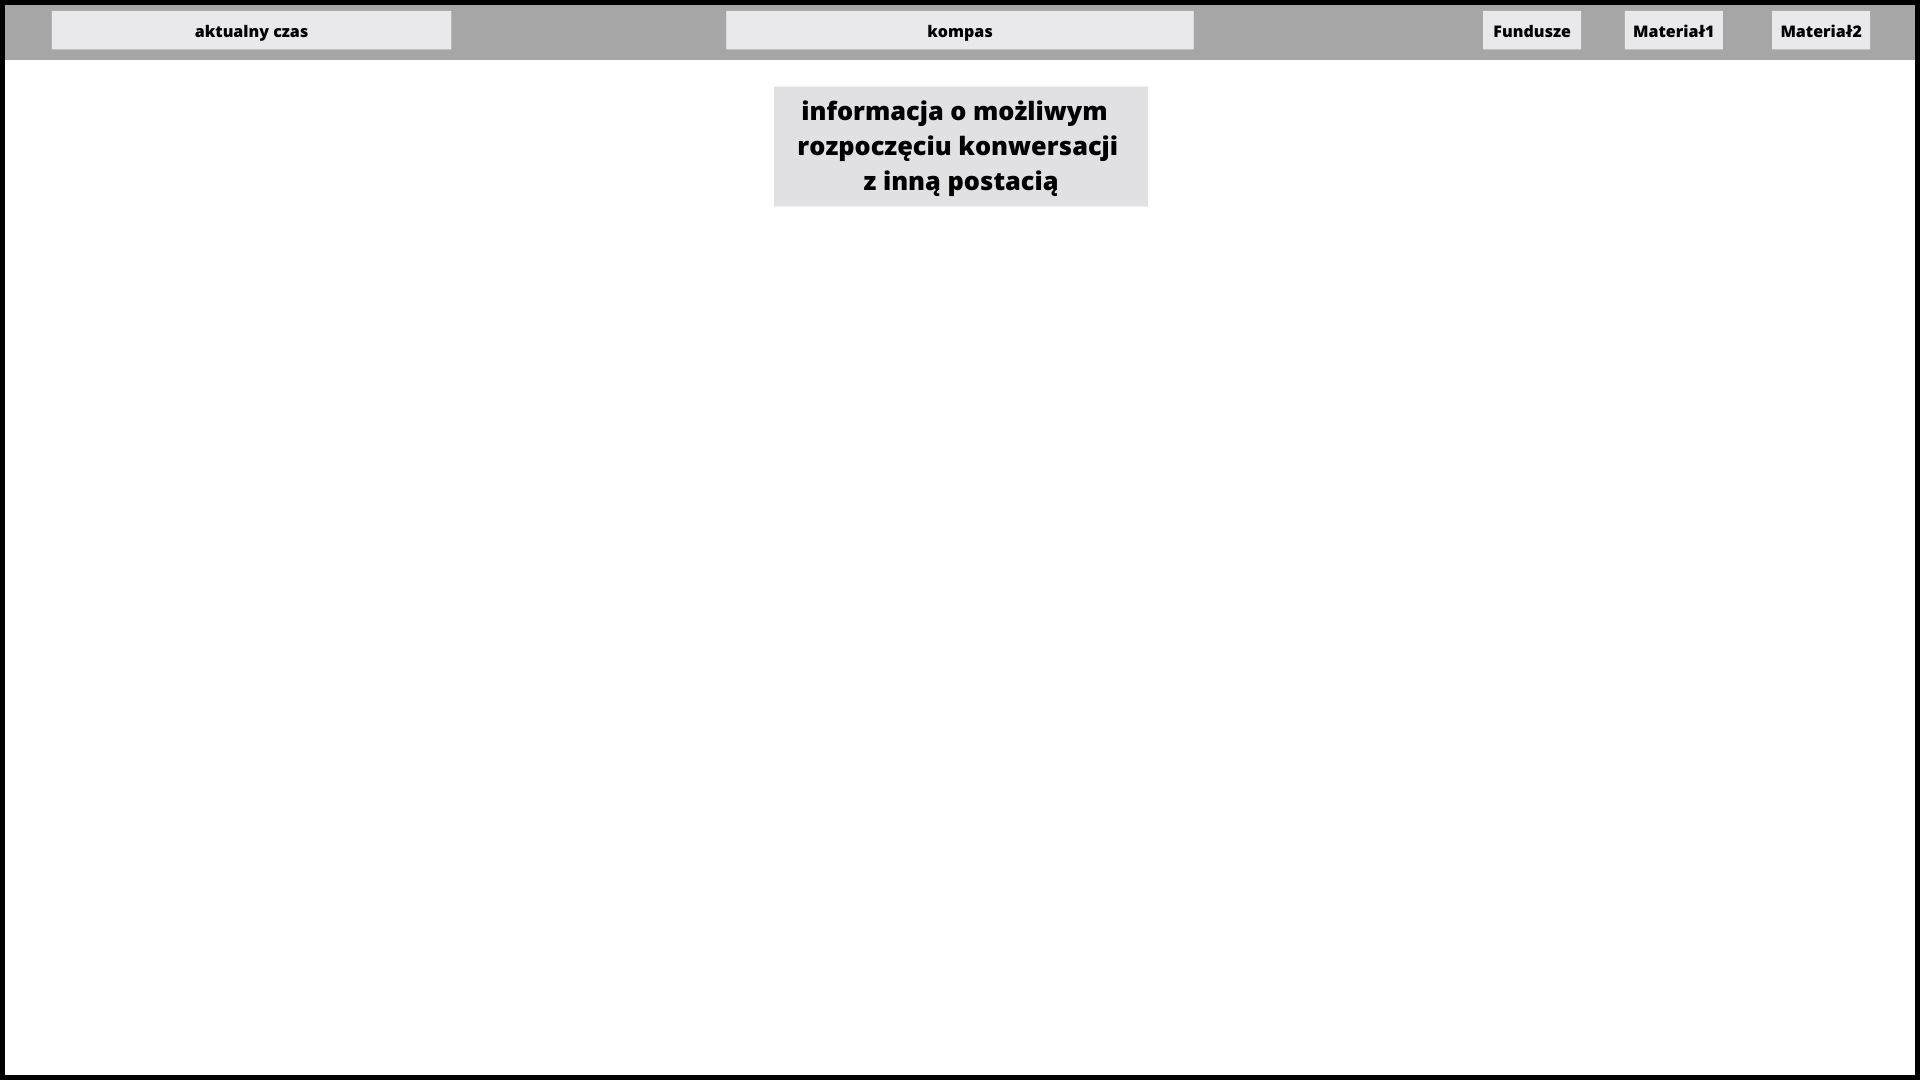
\includegraphics[width=0.9\textwidth]{images/ui/ui_proj_ogolne.jpg}
    \caption{Projekt interfejsu podstawowego UI.
    }\label{fig:ui_main}
\end{figure}
 
\subsection{Menu stawiania budynków}
 W menu stawiania budynków informacje wcześniej przedstawione zostaną na ekranie. Dodatkowo pokażą nam się dostępne do zbudowania budynki, a po wybraniu pojawią się przed nami. Po zatwierdzeniu budynek zostanie wybudowany.
	Inspiracją do przedstawienia dostępnych budowli jest rozwiązanie gry Orcs must die!


    Szacowany projekt trybu budowania UI wyświetlono na rysunku \ref{fig:ui_bud} .
    \begin{figure}[htbp]
        \centering
        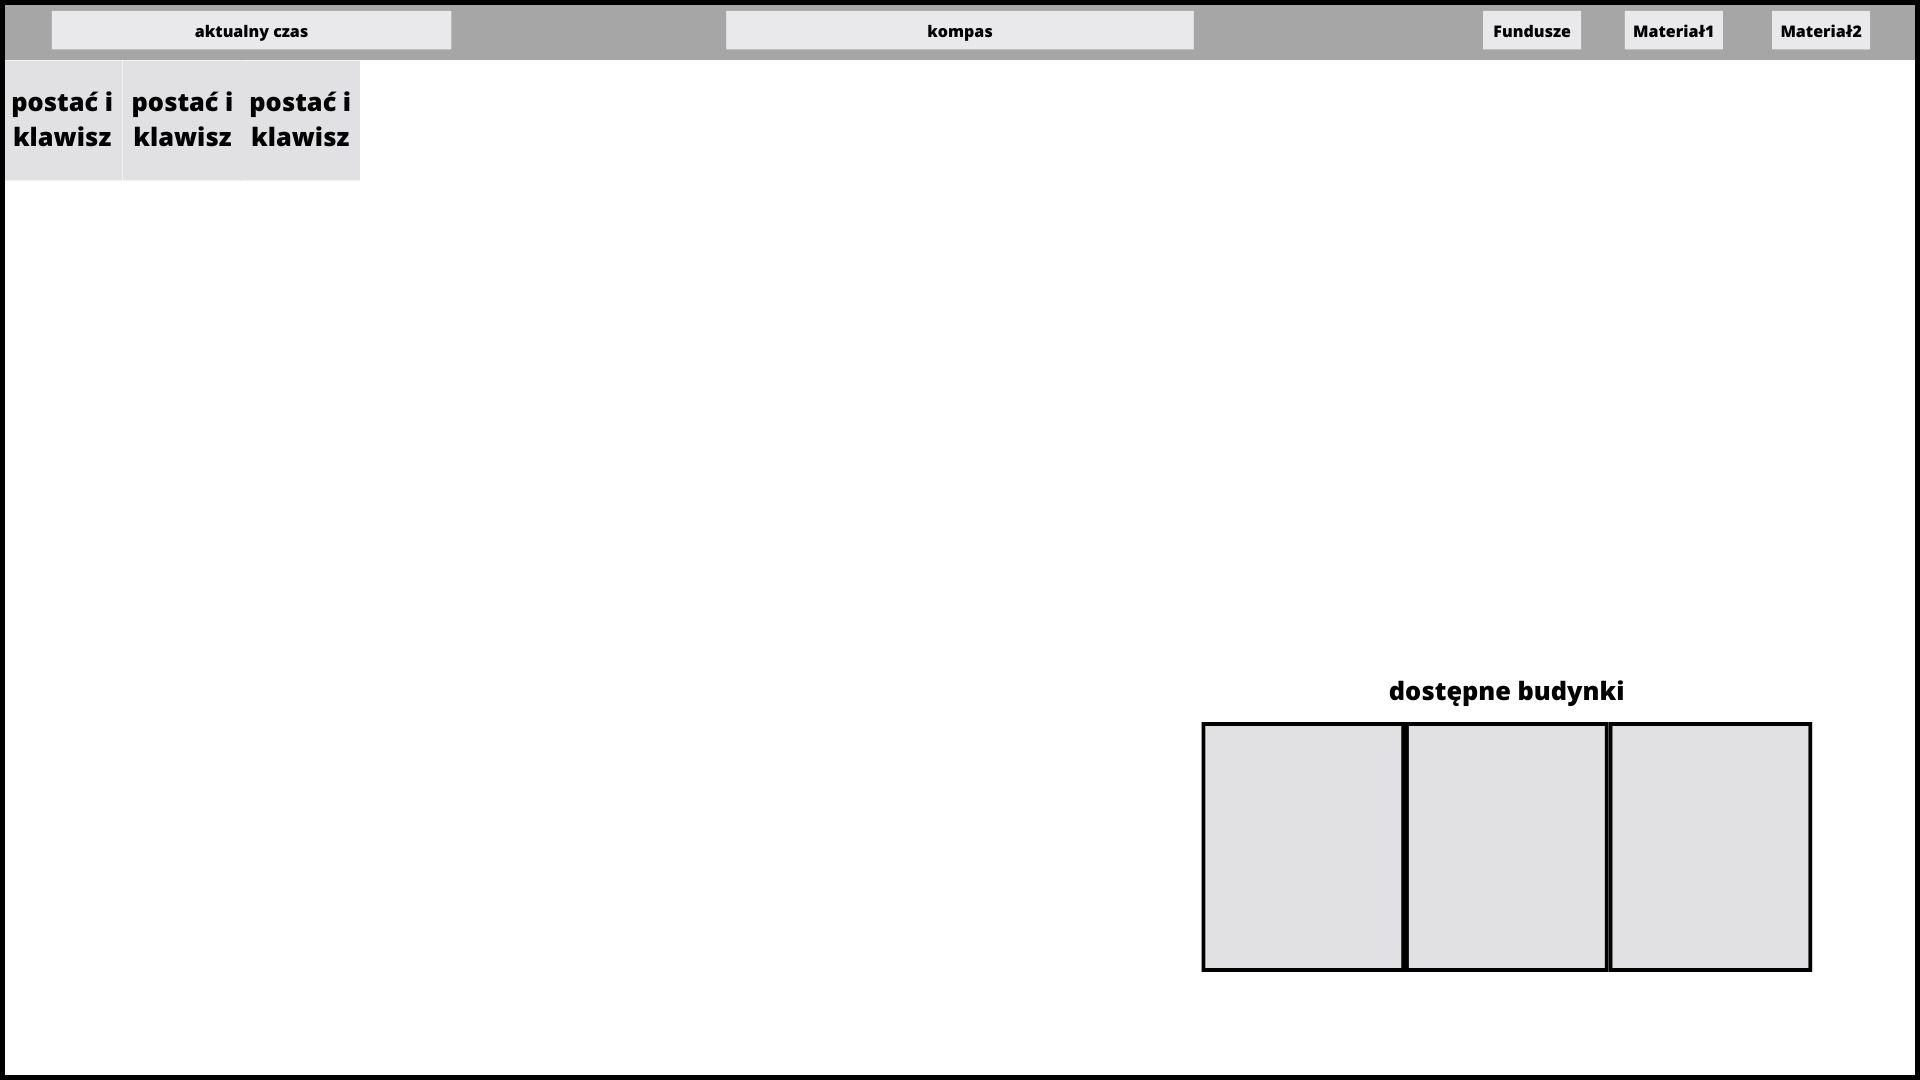
\includegraphics[width=0.9\textwidth]{images/ui/ui_proj_budowanie.jpg}
        \caption{Projekt menu stawiania budynków UI.
        }\label{fig:ui_bud}
    \end{figure}


\subsection{Tryb walki}
Bliźniaczo do trybu budowania, gdy rozpocznie się walka, podstawowe informacje zostają na ekranie, a dodatkowo gracz dostaje informacje o dostępnych rozkazach do wydania. Nasze rozwiązanie będzie podobne do pomysłu z gry Mount\&Blade.

Szacowany projekt trybu budowania UI wyświetlono na rysunku \ref{fig:ui_wal} .
    \begin{figure}[htbp]
        \centering
        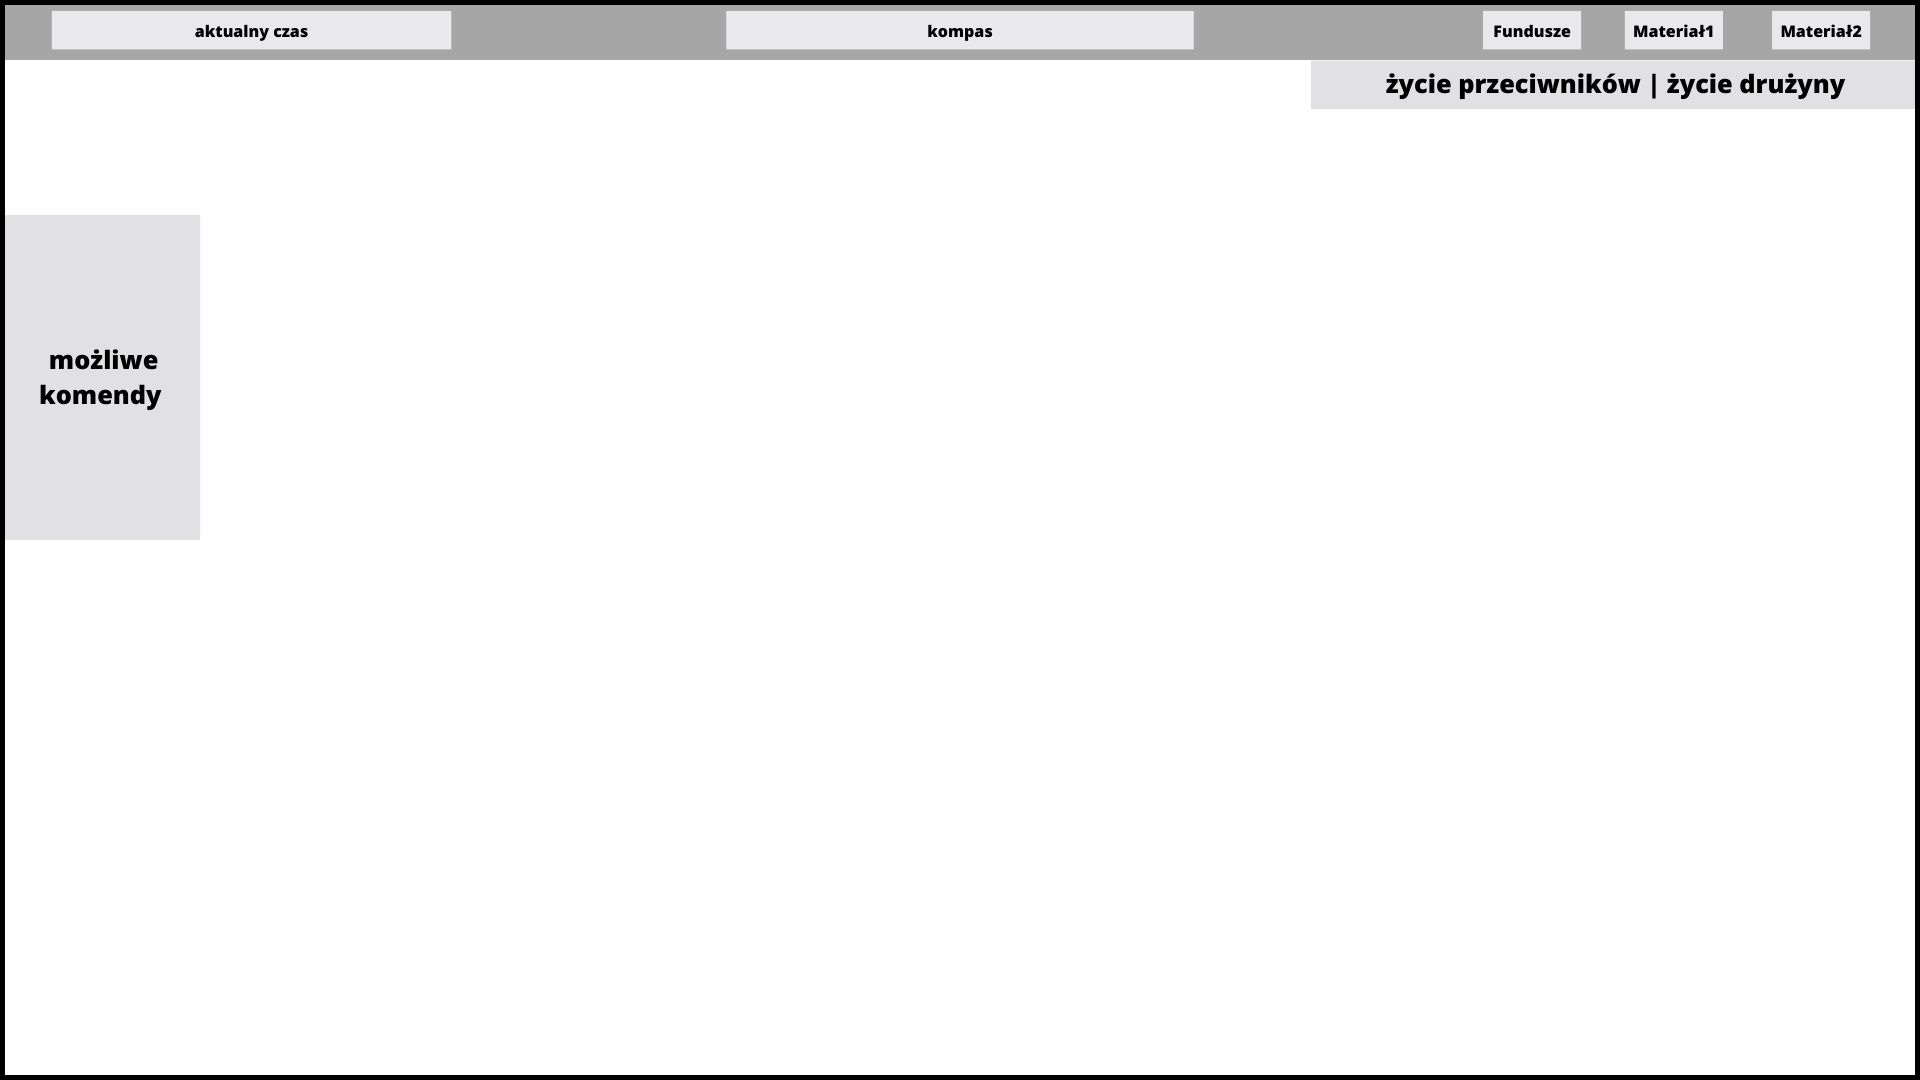
\includegraphics[width=0.9\textwidth]{images/ui/ui_proj_walka.jpg}
        \caption{Projekt trybu walki UI.
        }\label{fig:ui_wal}
    \end{figure}
